\documentclass{ligodoc}

\usepackage{graphicx}
\usepackage{amssymb}
\usepackage{amsmath}
\usepackage{longtable}
%\usepackage{rotating}
\usepackage[usenames,dvipsnames]{color}
%\usepackage{fancyhdr}
% Some PDFtex-specific options
\usepackage{hyperref}
\usepackage{subfigure}
\usepackage{bm}   %bold math
\usepackage{textcomp}     %non-italic mu
\newcommand{\micro}{\textmu{}}


\ligodccnumber{x}{xx}{xxxx}{xx}{x}
\ligodistribution{LIGO Scientific Collaboration}
\ligodraft

\title{GEO Squeezing Noise Budget}
\author{Kate Dooley, Hartmut Grote, Henning Vahlbruch (\emph{alphabetical order for now})}
%\date{Feb. 28, 2012}
\begin{document}


\section{Introduction}
This document serves as a summary of the current understanding of the
noise budget of the GEO squeezer. It includes the following:
\begin{itemize}
\item overview of the GEO squeezer setup
\item review of mechanisms by which the squeezing level as seen in h is affected
\item description of methods and results of measurements of the
  optical losses and phase noise
\item design and characterization of the control loops that intregrate
  the squeezer with the interferometer
\item suggestions for future work
\end{itemize}


\section{Overview of squeezing setup}
A description of the GEO squeezer itself can be found in
Ref. [Henning's 2010 Class. Quantum Grav. paper]. Coherent control
sidebands, Faraday isolator injection point, ... 



\section{Reductions to potential squeezing}
The amount of squeezing that can be achieved with an interferometer is
a function of three primary quantities:
\begin{enumerate}
\item level of injected squeezing
\item optical losses (including mode-matching and alignment)
\item phase noise
\end{enumerate}
Models are presented here and measurements follow in the next sections.


\subsection{Injected squeezing}
The level of injected squeezing is limited to the performance of the
squeezer itself. The level of squeezing generated by the squeezer can
be controlled during interferometer operations by changing the
setpoint for the Mach-Zehnder (MZ) in the squeezing box. A PZT on one
of the MZ mirrors changes the MZ length and therefore controls the
amount of green light transmitted through the MZ to match the
requested setpoint. This green pump field is sent directly into the
OPA cavity to generate the correlated 1064 nm photons. The degree of
squeezing is a non-linear function of the pump power and is plotted in
Figure~\ref{fig:sqz_generated} using the GEO squeezer parameters which
are found in Table~\ref{tab:GEOsqz_params}. This shows the upper
limits of our achievable squeezing level. A maximum pump power of 45
mW, or 11 dB of generated squeezing, may be used with the GEO
squeezer.

\begin{figure}
\begin{centering}
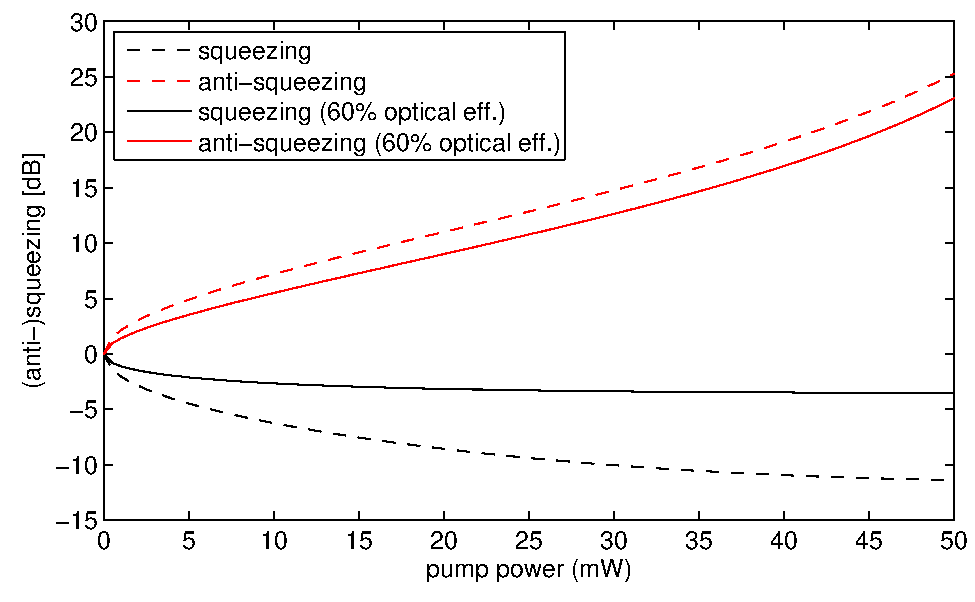
\includegraphics{/home/kadool/GEOHF/projects/sqz_generated.pdf}
\caption{The amount of generated squeezing and anti-squeezing as a
  function of the green pump power. An example of the effect of
  optical losses is included by showing the equivalent curves when the
  optical efficiency of the squeezer path is 60\%. No phase noise is
  included.}
\label{fig:sqz_generated}
\end{centering}
\end{figure}

\begin{table}
\centering
\caption{GEO squeezer parameters (see p.70, 90 Khalaidovski thesis).}
\begin{tabular}{l l}
\hline
squeezer breadboard optical efficiency & 93\% \\
OPO output coupler transmission & 8\%\\
OPO intracavity loss & 4\%\\
OPO round-trip length & 0.0186~m\\
frequency & 5~MHz\\
OPO threshold power & 60~mW\\
\hline
\end{tabular}
\label{tab:GEOsqz_params}
\end{table}


\subsection{Optical losses}
Any time the squeezed vacuum field experiences an optical loss, the
loss is replaced by the classic vacuum field:
\begin{equation}
V^\prime= VT + L
\end{equation}
Here, $V$ is the initial variance of the squeezed state, $T$ the optical
efficiency, and $L$ the optical losses, where
$T+L=1$. Figure~\ref{fig:sqzpumplosses} shows the how the degree of
squeezing is degraded as a function of optical efficiency for several
different pump powers.

\begin{figure}
\begin{centering}
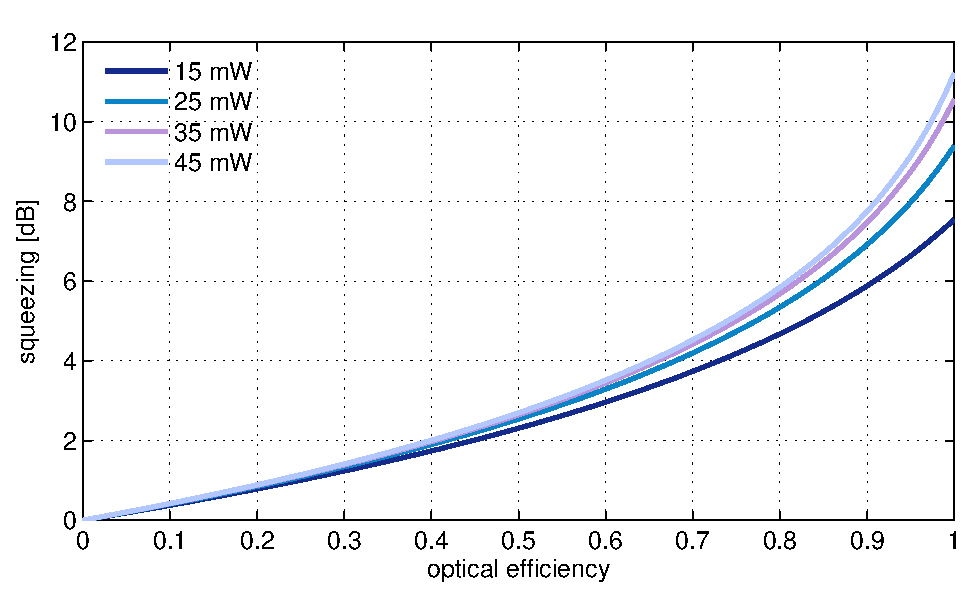
\includegraphics{/home/kadool/GEOHF/projects/sqz_pump_eff.pdf}
\caption{The expected amount of observed squeezing based on the green
  pump power and the optical efficiency of the squeezed field path. This
  model assumes no phase noise.}
\label{fig:sqzpumplosses}
\end{centering}
\end{figure}


\subsection{Phase noise}
Phase noise arises when there is relative motion between the angle of
the squeezing ellipse and the angle of the measurement quadrature of
the interferometer. The degree of (anti-)squeezing is reduced to the
following quantities for an rms phase noise of $\theta$:
\begin{eqnarray}
V_s^{\prime} =& V_s \cos^2{\theta} + V_a \sin^2{\theta} \\
V_a^{\prime} =& V_a \cos^2{\theta} + V_s \sin^2{\theta} 
\end{eqnarray}
where $V_a$ and $V_s$ are the variances of the anti-squeezed and
squeezed states, respectively, before including the effect of phase
noise. Note that for small $\theta$, the change in the (anti-)squeezed
states depends linearly on the degree of squeezing/anti-squeezing,
respectively. Given the amount of anti-squeezing is much greater than
the amount of squeezing (see Fig.~\ref{fig:sqz_generated}), the
squeezed state is much more significantly affected by phase noise than
the anti-squeezed state. Figure~\ref{fig:sqz_generated_noises} shows
how the squeezing as a function of pump power is reduced most
significantly at high pump powers (ie. where there are the highest
levels of anti-squeezing). Figure~\ref{fig:pump_phase} shows squeezing
as a function of phase noise for several pump powers when the optical
losses are 40\%. The highest pump power of 45~mW is only beneficial if
the total rms phase noise is less than 10~mrad.

\begin{figure}
\begin{centering}
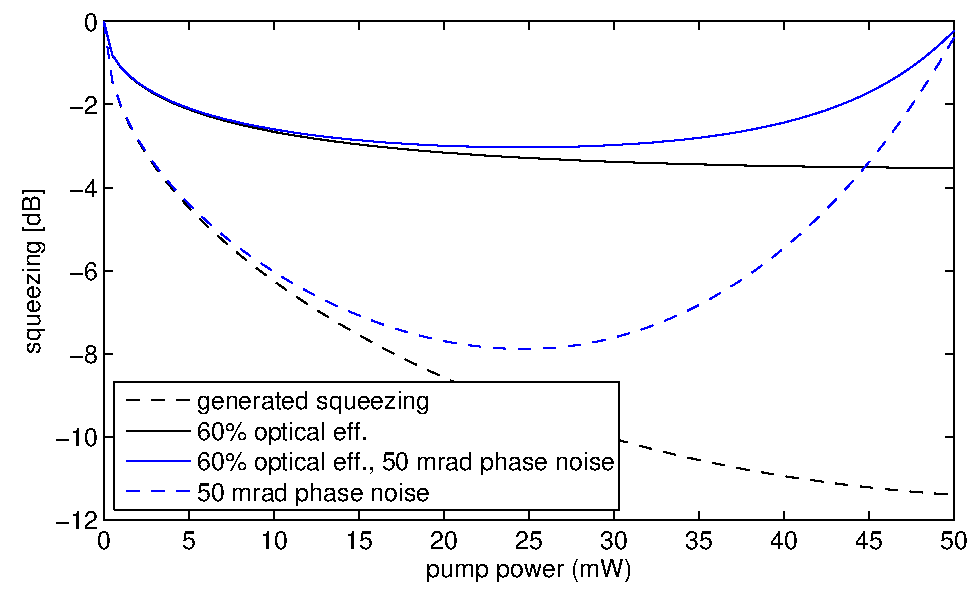
\includegraphics{/home/kadool/GEOHF/projects/sqz_generated_noises.pdf}
\caption{Generated squeezing as a function of the pump power (black
  dashed curve) shown in contrast with the equivalent curves that
  include 40\% optical losses and 50~mrad phase noise. These numbers
  are selected for demonstration purposes only.}
\label{fig:sqz_generated_noises}
\end{centering}
\end{figure}

\begin{figure}
\begin{centering}
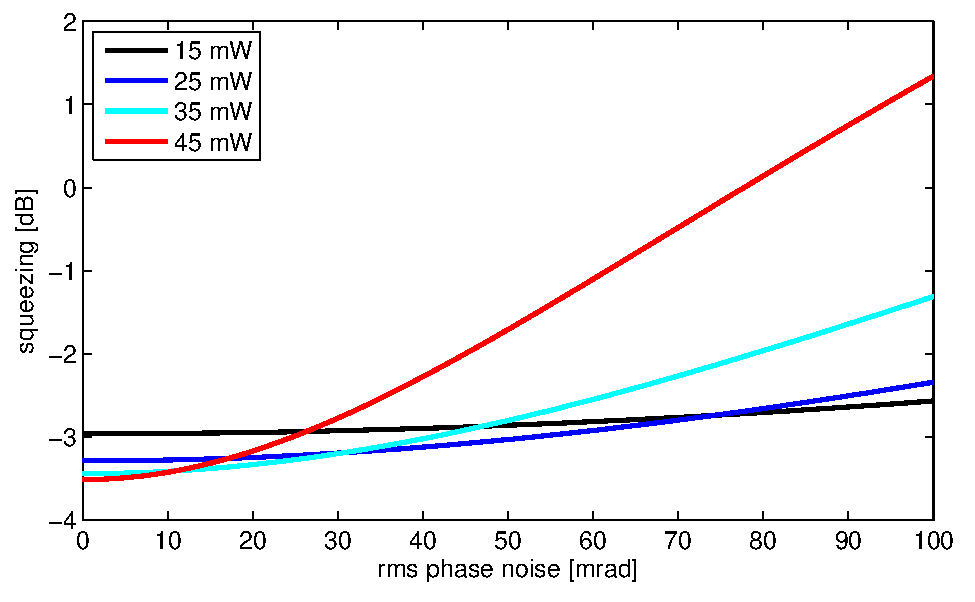
\includegraphics{/home/kadool/GEOHF/projects/pump_phase.pdf}
\caption{Squeezing as a function of phase noise for 4 different pump
  powers when optical losses are 40\%.}
\label{fig:pump_phase}
\end{centering}
\end{figure}



\section{Optical losses}
Table~\ref{tab:losses} summarizes our optical loss budget for the
squeezer path. We find that only 63\% of the squeezed light sent into
the interferometer makes it to the detection PD. With the nominal 35 mW pump power, or 10.5 dB injected squeezing, these optical losses alone reduce the maximum possible level of achieved squeezing to 3.7 dB. 

\begin{table}
\centering
\caption{Optical losses of squeezed beam. The resulting transmission
  upon multiplying the optical efficiencies in series is 63\%.}
\begin{tabular}{l l l l} %r@{}l r@{}l
\hline
component & power loss & comment \\
\hline
squeezer path Faraday & 3.3\% & 1.5\% \\
output port Faraday & 3.3\% $\times$ 2 & guess \\
BDO1 transmission & 1\% $\times$ 2 & \\
SR cavity (when locked) & 1\% & above 1 kHz \\
OMC mode-matching loss & 6\% & \\
squeezer mode-matching loss & 2\% & \\
OMC AR coating loss & 1\% & \\
OMC internal losses & 14\% & deduced from other measurements \\
OMC trans PD detection loss & 9\% & Perkin-Elmer \\
\hline
\end{tabular}
\label{tab:losses}
\end{table}

\begin{figure}
\begin{centering}
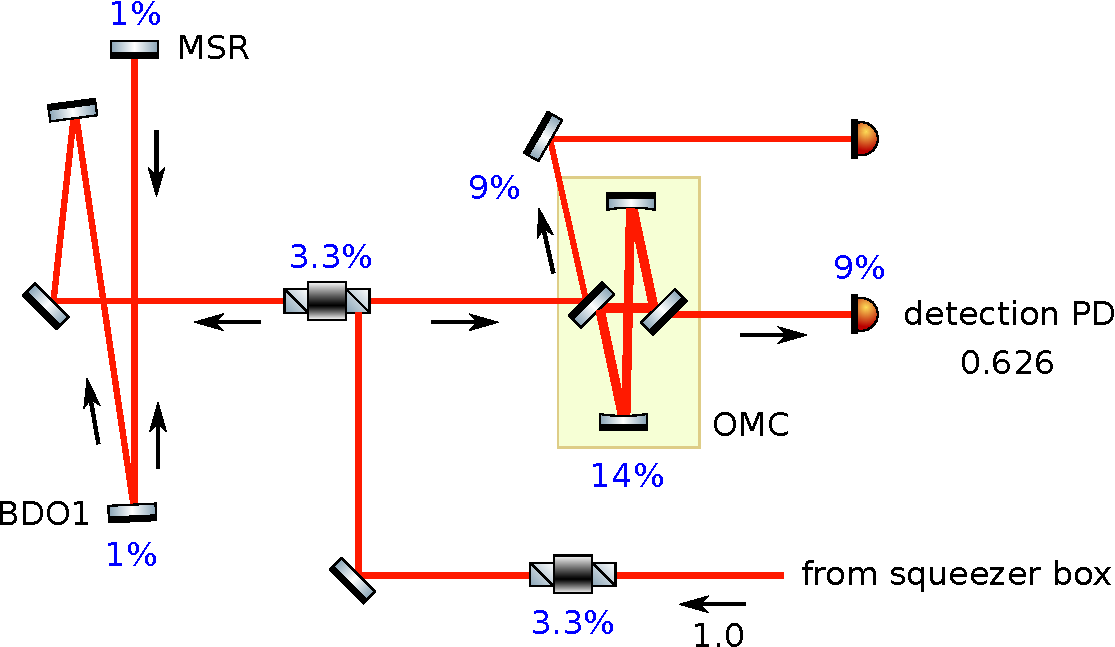
\includegraphics[width=0.8\textwidth]{/home/kadool/figures/opticallosses.pdf}
\caption{Optical losses in the squeezer path.}
\label{fig:powerbudget}
\end{centering}
\end{figure}

The single greatest source of loss is the OMC and second is the
detection PD. The OMC is known to have excessive losses due to poor AR
coatings and most likely dirty mirrors and can in principle be easily
improved with new optics. The current Perkin-Elmer photodiode is also
a high-loss component that can be replaced with a much better
specimen. The polarizing beam splitters of the Faraday isolators each
have approximately $1\%$ loss and with investigation into better
polarizers, may be improved. Details of short-term goals for
improvement of optical efficiency are found in
Section~\ref{sec:future}.


\subsection{Mode-matching}
The mode-matching lenses used to match the squeezed field into the OMC
were selected based on a model, and then tuned in-situ. The bright
alignment beam was used and the OMC scanned to look for minimizing the
TEM02/20 mode. The mode-matching is approximately 98\%.


\subsection{Alignment}
The squeezed field needs to be aligned to the carrier field at the
inteferometer output port. There are several ways of generating an
alignment signal, all of which use the squeezer coherent control
sidebands. The true alignment signal is the beat between the carrier
TEM00 and CCSB TEM01/10. However, most of the carrier light at the
output port is made of higher order modes which add noise to the
measurement. Because the Michelson sidebands are spatially cleaner at
the output port than the carrier (and should be aligned to the
carrier), they serve as a potential alignment signal candidate. A
summary of the options explored for generating an alignment signal are
found in Table~\ref{tab:AA}.

\begin{table}
\centering
\caption{Options for generating an alignment error signal.}
\begin{tabular}{l l l}
\hline
where & what & frequency \\
\hline
OMC REFL QPD &     CCSBs vs. MI RF SBs & 300 kHz \\
FAR camera &          CCSBs vs. carrier & 15.2 MHz \\
FAR camera &        CCSBs vs. MI RF SBs & 300 kHz \\
\hline
\end{tabular}
\label{tab:AA}
\end{table}

\textcolor{blue}{Include plot of first results.}


\section{Phase noise}
The squeezing ellipse orientation must match the angle of the
interferometer output field to make the best use of the squeezed
field. The interferometer output field is ideally made up of only the
local oscillator for the gravitational-wave signal, the dark fringe
offset. However, in practice, other light is present and contributes
to the shot noise at the detector. The power of squeezing is that it
can reduce the shot noise of the light at the output port, no matter
what it is made of. Therefore, the sum of the phase jitters of all
fields must be considered. In addition, it should be pointed out that
only the rms phase noise matters, not the shape of the frequency
content.


\subsection{Phase noise sensing and control}
There are several options for how to implement a squeezer longitudinal
phase servo. First, there are four choices for how to generate such
an error signal:
\begin{itemize}
\item carrier against CCSBs in OMC trans (OMC can't have too high a finesse!)
\item carrier against CCSBs at pick-off before OMC
\item MI RF SBs against CCSBs in OMC refl
\item MI RF SBs against CCSBs at pick-off before OMC
\end{itemize}
We are currently using option 4, and will soon have the electronics to
test out option 1.

Second, there are choices for how to feedback a control signal:
\begin{itemize}
\item add to 80 MHz frequency generator used for demodulation of
  sqz. to GEO laser PLL loop
\item PZT in the squeezer injection path
\end{itemize}


Our current setup for creating a squeezer to GEO output relative phase
error signal uses the beat of the squeezer sidebands with the
Michelson sidebands in reflection of the OMC which are at 15.2~MHz and
14.9~MHz, respectively. A sample error point spectrum is shown in
Figure~\ref{fig:sqzEP} and demonstrates that we measure only 5 mrad
rms residual phase noise. We also inject a line at 6500 Hz to monitor
the signal-to-noise of the error signal.

\begin{figure}
\begin{centering}
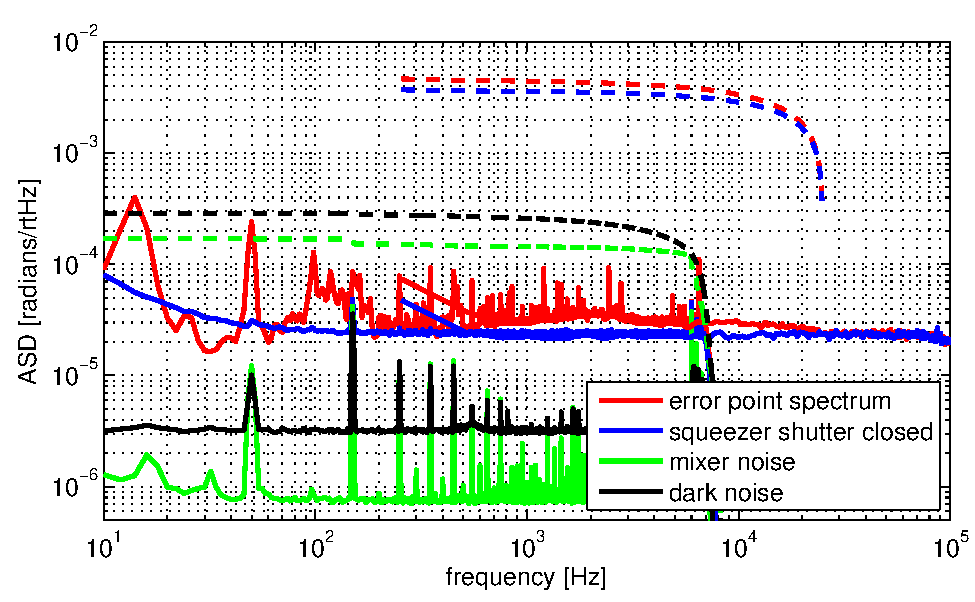
\includegraphics{/home/kadool/GEOHF/2012/03/17/sqzEP_seminar.pdf}
\caption{Calibrated squeezer phase error point (red curve), measured
  as the beat between the squeezer control sidebands and the RF
  Michelson sidebands in reflection of the OMC. This loop operates
  with a bandwidth of about 1 kHz and is limited by sensor/shot (blue
  curve) above 25~kHz. The servo is not gain-limited because the
  spectrum is so flat such that little to no improvement in rms
  noise is to be gained by increasing the gain. The residual rms phase
  noise is 5 mrad.}
\label{fig:sqzEP}
\end{centering}
\end{figure}





\subsection{Noiselock}
We implement a slow servo called the \emph{noiselock loop} that serves
to change the squeezing quadrature in order to maximize the strain
sensitivity. The demodulation phase of the longitudinal phase error
signal is dithered at 11.6~Hz and a band-limited root-mean-square of
strain is then demodulated at this dither frequency and a control
signal derived. A schematic of the servo is in
Figure~\ref{fig:noiselockservo}. The underlying causes for slow phase
drift is not understood at this time. An example of how much drift we
observe is shown in Figure~\ref{fig:noiselock}.

\begin{figure}
\begin{centering}
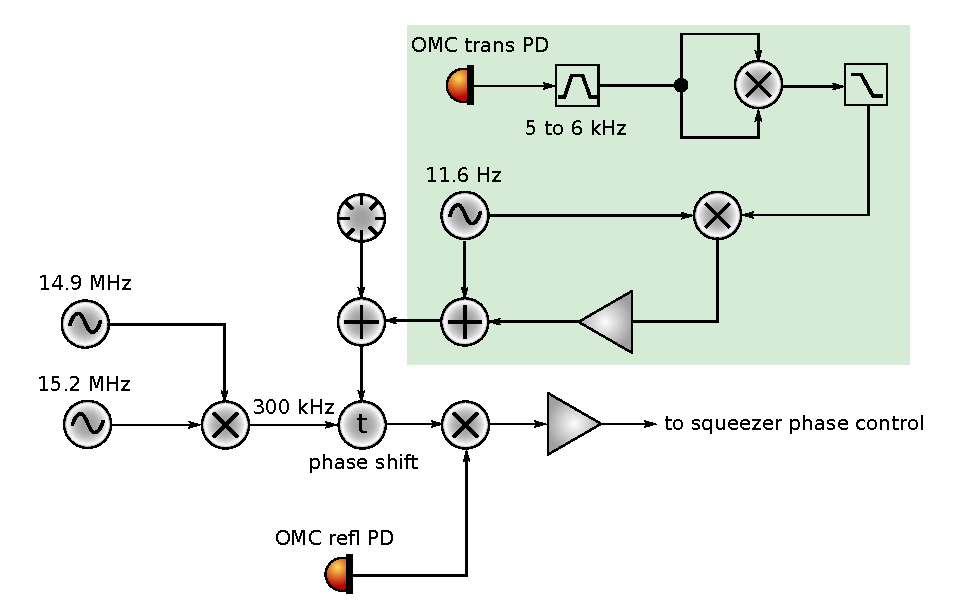
\includegraphics[width=0.9\textwidth]{/home/kadool/figures/noiselock_servo.pdf}
\caption{Schematic of the noiselock servo. The demodulation phase of
  the squeezing angle error signal is modulated at $f_0=11.6$ Hz. The
  band-limited rms of interferometer strain is in turn demodulated at
  $f_0$ and a derived control signal is in turn sent to the
  demodulation phase of the squeezing angle error signal.}
\label{fig:noiselockservo}
\end{centering}
\end{figure}


\begin{figure}
\begin{centering}
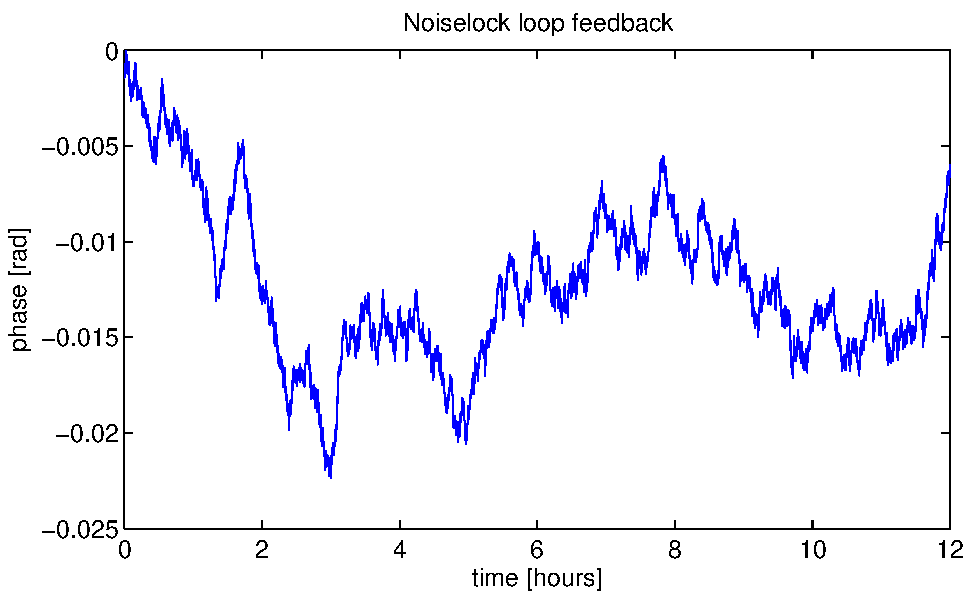
\includegraphics[width=\textwidth]{/home/kadool/GEOHF/2012/03/16/noiselock_FPcal.pdf}
\caption{Example of drift of squeezer demodulation phase over the
  course of 12 hours.}
\label{fig:noiselock}
\end{centering}
\end{figure}



\subsection{RF frequencies}
This section is based on work from LIGO T0900325 and evaluates the
role of the RF sidebands in generating phase jitter of the
interferometer output field. Understanding the phase noise
contribution from the RF sidebands is important both because the
contribution can be large and because the squeezing ellipse
orientation cannot follow at these frequencies. Phase noise due to the
RF sidebands may, however, be reduced, as will be discussed shortly.

The dominant fields at the interferometer output port are those from
the dark fringe offset, the contrast defect, and the RF sidebands. The
dark fringe offset is the local oscillator for the gravitational-wave
sidebands in a DC readout configuration and is generated by holding
the Michelson arms slightly off of the dark fringe at the
anti-symmetric port. The contrast defect is light that makes it to the
anti-symmetric port due to asymmetry in the reflectivity of each
Michelson arm. The RF sidebands are ideally filtered by the OMC, but
due to limited finesse, some percentage is transmitted.

One of two effects of the RF sidebands on phase jitter comes from the
fact that the Michelson interferometer rotates the differential
carrier field by $90^\circ$, but leaves all other fields the same
(including the RF sidebands and the contrast defect). The result is
that at the output port, as shown in Figure~\ref{fig:AMPM}, the RF
sidebands are amplitude modulation (AM) of the dark fringe offset, yet
continue to be phase modulation (PM) of the contrast defect.

\begin{figure}
\begin{centering}
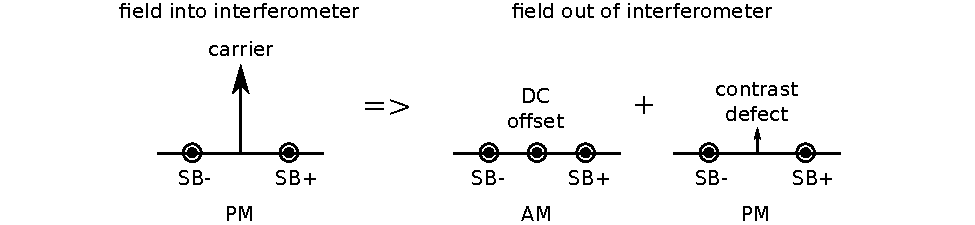
\includegraphics{/home/kadool/figures/AMPM.pdf}
\caption{The RF sidebands (SB+ and SB-) are generated via phase
  modulation of the carrier field. The Michelson interferometer
  rotates the differential carrier field by $90^\circ$, but leaves all
  other fields the same, including the RF sidebands and the contrast
  defect. The result is that at the output port, the RF sidebands are
  amplitude modulation (AM) of the dark fringe offset, yet continue to
  be phase modulation (PM) of the contrast defect.}
\label{fig:AMPM}
\end{centering}
\end{figure}

Because the squeezing quadrature is determined by the sum of the
fields at the interferometer output, both AM of the dark fringe offset
and PM of the contrast defect affect the angle that the squeezing
ellipse orientation must be matched to. Figure~\ref{fig:sqzquad} shows
phasors depicting these two situations. Should the ratio of dark
fringe offset to contrast defect amplitude be large, these effects are
reduced.

\begin{figure}
\begin{centering}
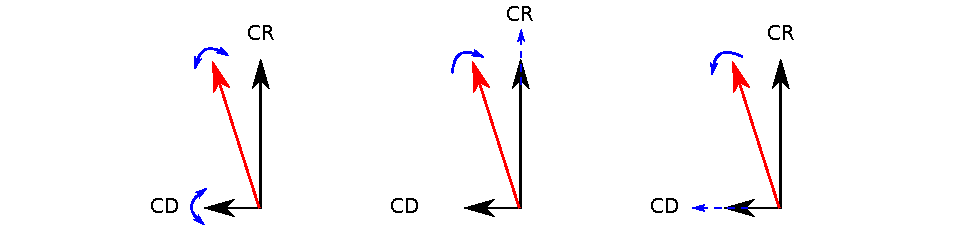
\includegraphics{/home/kadool/figures/SQZquadrature.pdf}
\caption{Examples of how jitter of the squeezing quadrature is
  generated. \textcolor{blue}{replace!}}
\label{fig:sqzquad}
\end{centering}
\end{figure}

The second effect of the RF sidebands on phase jitter arises when the
upper and lower sidebands are unequal in amplitude. Rather than
produce pure AM on the DFO and PM on the CD, there is some component
of PM on the DFO and AM on the CD.

In summary, changes in the interferometer output phase at RF
frequencies are created in four ways:
\begin{itemize}
\item phase noise of the contrast defect
\item amplitude noise of the dark fringe offset 
\item phase noise of the dark fringe offset due to unequal RF sideband amplitudes 
\item amplitude noise of the contrast defect due to unequal RF sideband amplitudes \textcolor{blue}{(true?)}
\end{itemize}
and may be expressed mathematically as in Eq. 90 from T0900325: 
%the rms fluctuation of the squeezing quadrature angle,
%$\Gamma_{\mathrm{rms}}$, is dependent on the ratio of carrier light
%with signal, $P_{\mathrm{CR}}$, to light without signal that is
%transmitted through the OMC. Examples are the contrast defect carrier,
%$P_{\mathrm{CD}}$, and the sidebands, $P_{\mathrm{SB}}$:
\begin{equation}
\Gamma_{\mathrm{rms}} = \sqrt{\frac{P_{\mathrm{SB}}}{P_{\mathrm{CR}}} \left( \frac{1}{\eta} + \epsilon^2 \frac{\eta-1}{\eta} \right)}
\label{eq:Gammarms}
\end{equation}
All powers in this equation are for those transmitted through the OMC,
and the variables $\eta$ and $\epsilon$ are defined as follows:
\begin{equation}
\eta = \frac{P_{\mathrm{CR}}}{P_{\mathrm{CD}}}
\end{equation}
\begin{equation}
\epsilon = \frac{1}{2}\frac{P_{\mathrm{SB+}}-P_{\mathrm{SB-}}}{P_{\mathrm{SB+}}+P_{\mathrm{SB-}}}
\end{equation}


The sideband imbalance is quantified by $\epsilon$ and a sample
measurement of the imbalance is shown in
Figure~\ref{fig:modescan}a. Currently, $\epsilon=0.06$. The contrast
defect, commonly quoted as $1/\eta$, can be measured by comparing the
power transmitted through the OMC with and without the dark fringe
offset. It accounts for approximately 5\% of the power at the output
port, as seen in Figure~\ref{fig:modescan}b.

\begin{figure}
\begin{centering}
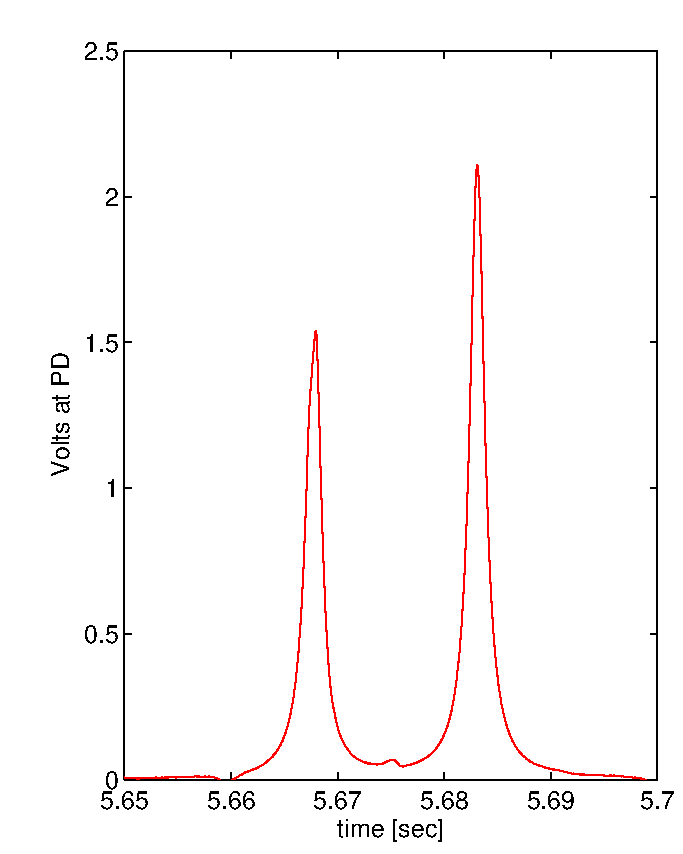
\includegraphics[width=0.5\textwidth]{/home/kadool/GEOHF/projects/modescan/sidebands.pdf}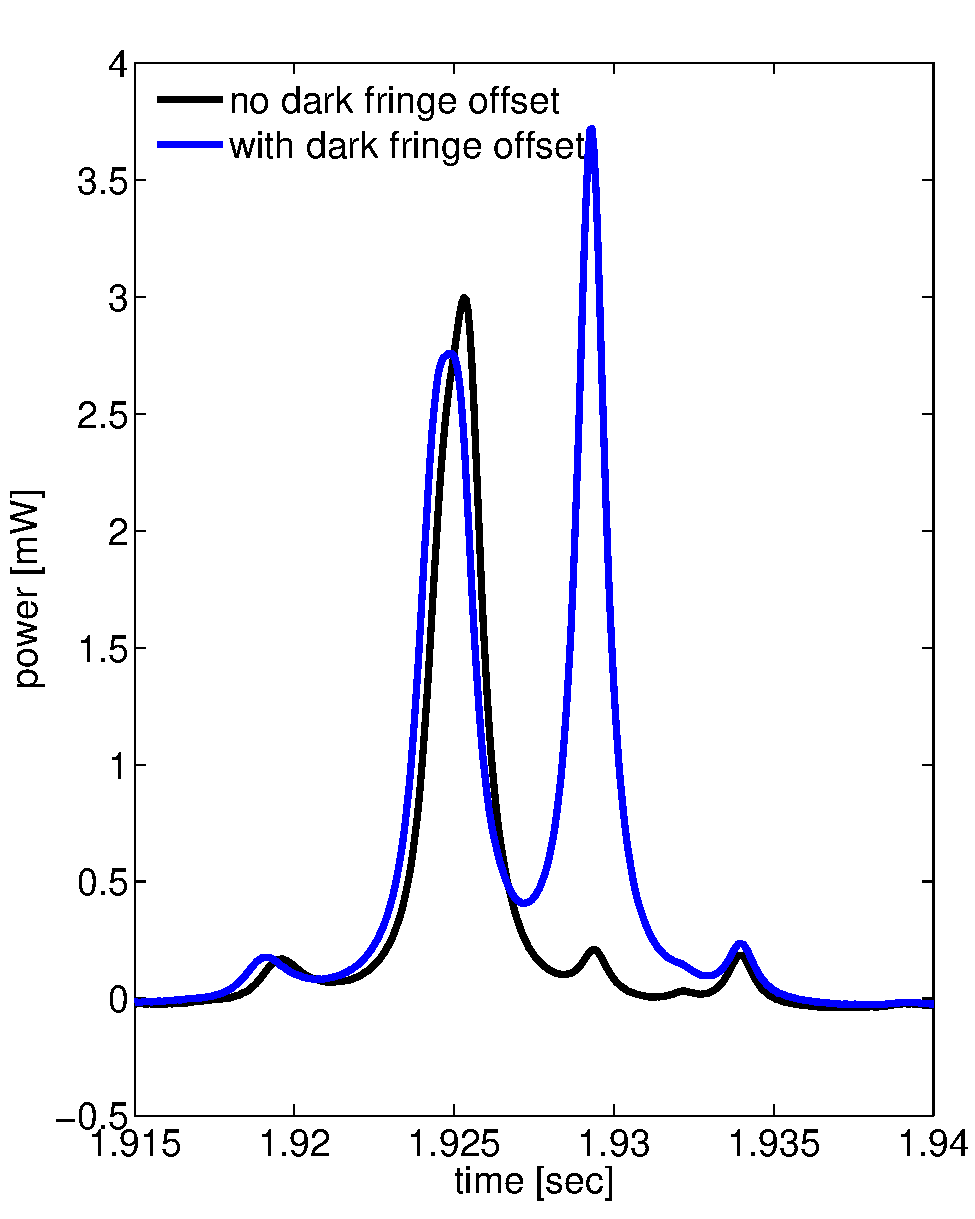
\includegraphics[width=0.5\textwidth]{/home/kadool/GEOHF/projects/modescan/DFO_noDFO.pdf}
%\includegraphics[width=0.5\textwidth]{/home/kadool/GEOHF/projects/modescan/contrastdefect.pdf}
\caption{Mode scan of the output port. The left-hand plot shows the
  Michelson RF sideband imbalance. A higher-order carrier mode sits on
  top of the lower sideband, so this figure is created by subtracting
  the carrier content. The imbalance is $\epsilon = 0.06$. The
  right-hand plot shows the ratio of contrast defect to carrier power
  for our typical dark fringe offset. The ratio is about 0.05. The
  sideband amplitude is reduced by a factor of 4.4 from fall 2011 and
  is the new standard.}
\label{fig:modescan}
\end{centering}
\end{figure}

Figure~\ref{fig:phirms} shows the dependence of phase noise on
contrast defect for our current sideband imbalance. This uses
$P_{CR}=1.6$ and $P_{MI\_SB+}=0.08 T_{MI}$ (for the $4.4\times$
sideband amplitude reduction). We estimate the signal recycling cavity
sideband amplitude as $P_{SR\_SB+}=0.02 T_{SC}$. Note $T_{MI}$ and
$T_{SR}$ are calculated in Table~\ref{tab:OMCparams}. We explored the
effect of these factors on observed squeezing by changing the rms
phase noise up to a factor of 4.4 by reducing the sideband
amplitude. We also tried increasing the dark fringe offset. 
%an improvement in the
%observed squeezing from 1.9~dB to 2.8~dB.


\begin{figure}
\begin{centering}
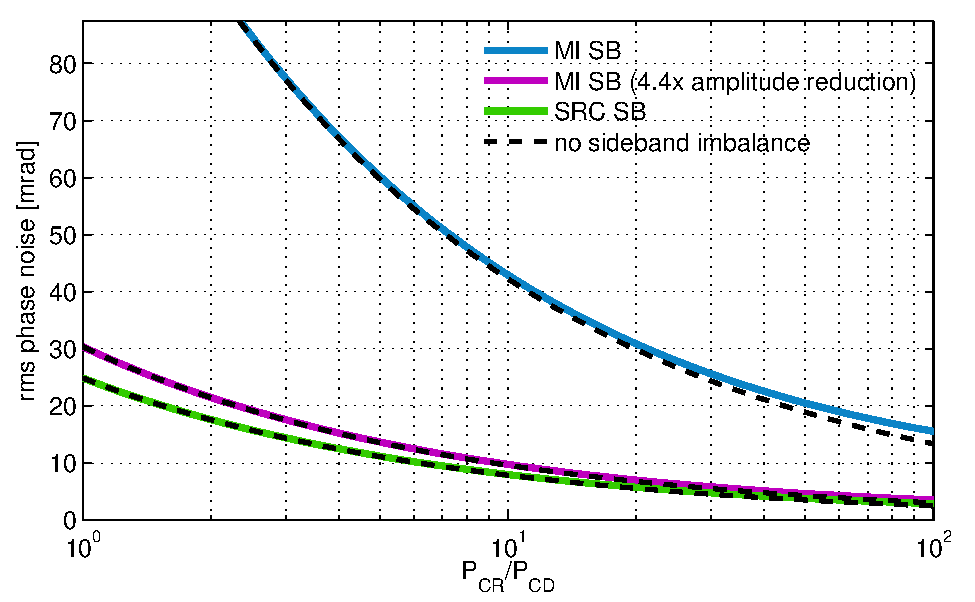
\includegraphics[width=1.1\textwidth]{/home/kadool/GEOHF/projects/SQZRFphase/RFrmsphase.pdf}
\caption{RMS phase noise as a function of the ratio of DC offset light
  to contrast defect light in the OMC transmitted beam. The typical
  operating point for GEO is $P_{\mathrm{CR}}/P_{\mathrm{CD}}=20$,
  which corresponds to an RMS phase noise for the Michelson sidebands
  of 6.7 mrad and 5.5 mrad for the SRC sidebands. The quadrature sum
  is 8.7 mrad.}
\label{fig:phirms}
\end{centering}
\end{figure}



\subsection{Higher order modes}
Role?
%We plan to test the effect of higher order modes on the squeezing
%quadrature jitter by placing an aperture in the beam path after the
%OMC.

%Based on the OMC finesse, $g$-factor and FSR, we can calculate the
%amount of higher order modes that are
%transmitted. Table~\ref{tab:HOMtrans} shows that of the first 5 HOMs,
%$n+m=5$ sits closest to the fundamental mode and $0.06\%$ of what's
%incident on the OMC is transmitted. Note that this does not reflect
%any coupling of higher order modes into the OMC fundamental mode as a
%result of poor alignment.

%We can place an upper limit on the contribution of higher order modes
%to squeezer phase noise through experiments with changing the sideband
%and dark fringe offset powers.


%\begin{table}
%\centering
%\caption{OMC mode spacing}
%\begin{tabular}{l| l l l l l}
%\hline
%HOM order ($n+m$) & 1 & 2 & 3 & 4 & 5 \\
%transmission factor (\%) & 0.041 & 0.014 & 0.011 & 0.016 & 0.061 \\
%\hline
%\end{tabular}
%\label{tab:HOMtrans}
%\end{table}



\subsection{Total known phase noise}
Taking the measured and anticipated rms phase noises at different
frequencies and adding them incoherently, we find that we have a total
known phase noise of 10 mrad rms. The summary of phase noises is shown
in Table~\ref{tab:phasenoises}.

\begin{table}
\centering
\caption{Measured and calculated phase noises. The quadrature sum is
  10 mrad rms.}
\begin{tabular}{l l l}
\hline
source & rms phase [mrad]\\
\hline
error point & 5 \\
14.9 MHz sidebands & 6.7 \\
9 MHz sidebands & 5.5 \\
\hline
\end{tabular}
\label{tab:phasenoises}
\end{table}


\subsubsection{Measuring total phase noise}
We currently do not have information about the rms phase noise between
audio and RF frequencies. We can indirectly determine what it is by
measuring the total phase noise via its affect on the squeezing
level. We can measure the total rms phase noise by mapping out the
curve of Figure~\ref{fig:sqz_generated_noises}. However, this will be
difficult if the total phase noise happens to be very small ($< 10$
mrad) because then the effect of phase noise is only measurable at
very high pump powers. At the moment, we are limited to at most
approximately 35~mW pump power and we know of only approximately
10~mrad phase noise. A method of putting an upper limit on the total
phase noise is to purposefully increase it by a known amount
(i.e. keep amplitude of MI RF sidebands at nominal locking level) and
measure the squeezing versus pump power curve. A first set of
measurements are shown in Figure~\ref{fig:sqzpump}. Our optical loss
budget predicts only 40\% losses and our known phase noises amount to
10 mrad, but this data is more consistent with 50\% optical losses and
70 mrad phase noise.

\begin{figure}
\begin{centering}
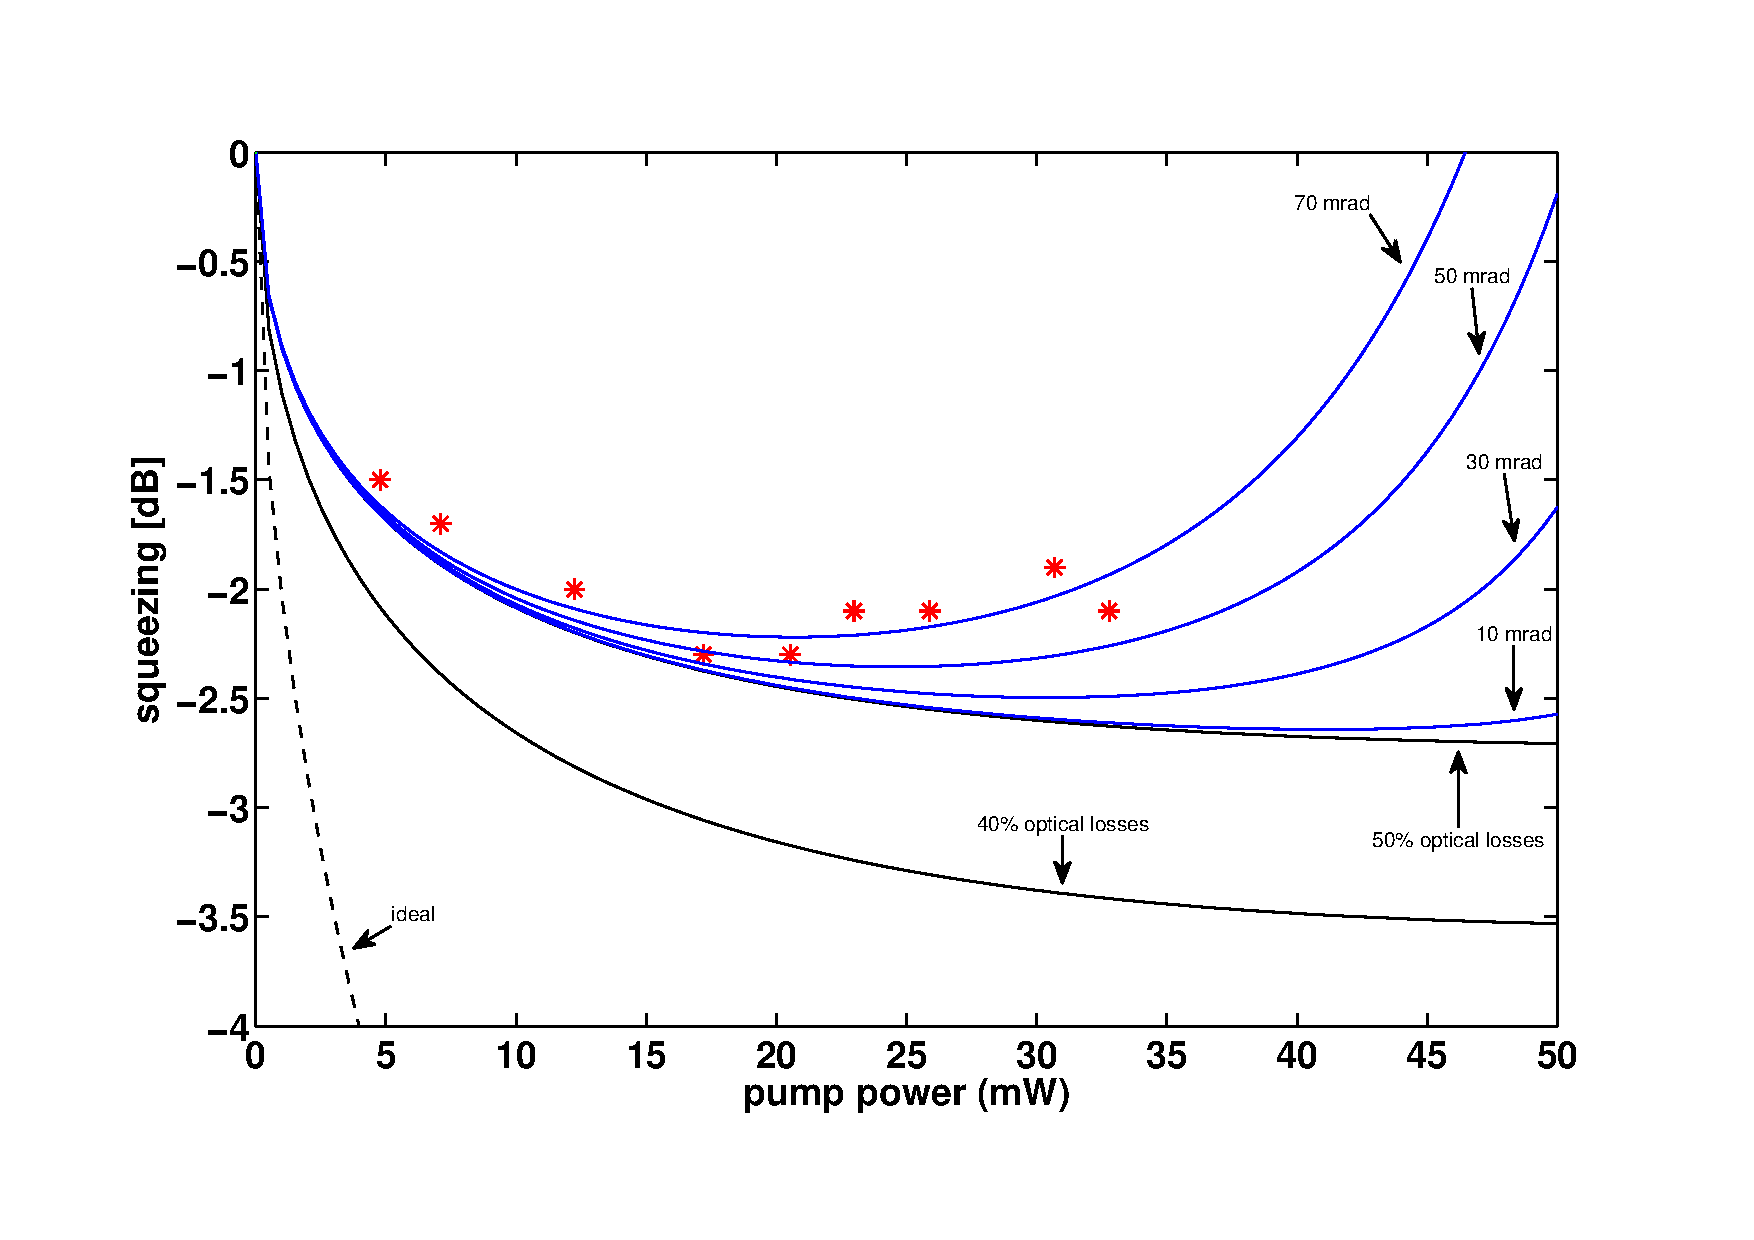
\includegraphics[width=1.0\textwidth]{/home/kadool/GEOHF/2012/07/06/sqz_pump.pdf}
\caption{First look at a measurement of squeezing vs. pump power.}
\label{fig:sqzpump}
\end{centering}
\end{figure}



\section{Expected observed squeezing}
Based on our measurements of the optical losses and phase noise, we
can predict the best possible achieveable squeezing level with the
interferometer output. With a green pump power of about 17 mW such
that the injected squeezing level is 8 dB and with 37\% losses, the
best squeezing possible is 3.2 dB. Phase noise of 10 mrad has a
negligible effect. As of early March, we measured 2.9 dB, leaving a
0.3 dB gap, which in fact is explained by other contributing noise
sources at high frequencies such as dark noise and laser amplitude
noise. Figure~\ref{fig:HFnoises} shows an example of these other
noise levels as of mid-April. This full accounting of observed
squeezing is not always realized, however. Since mid-April, for
example, there remains a gap.

\begin{figure}
\begin{centering}
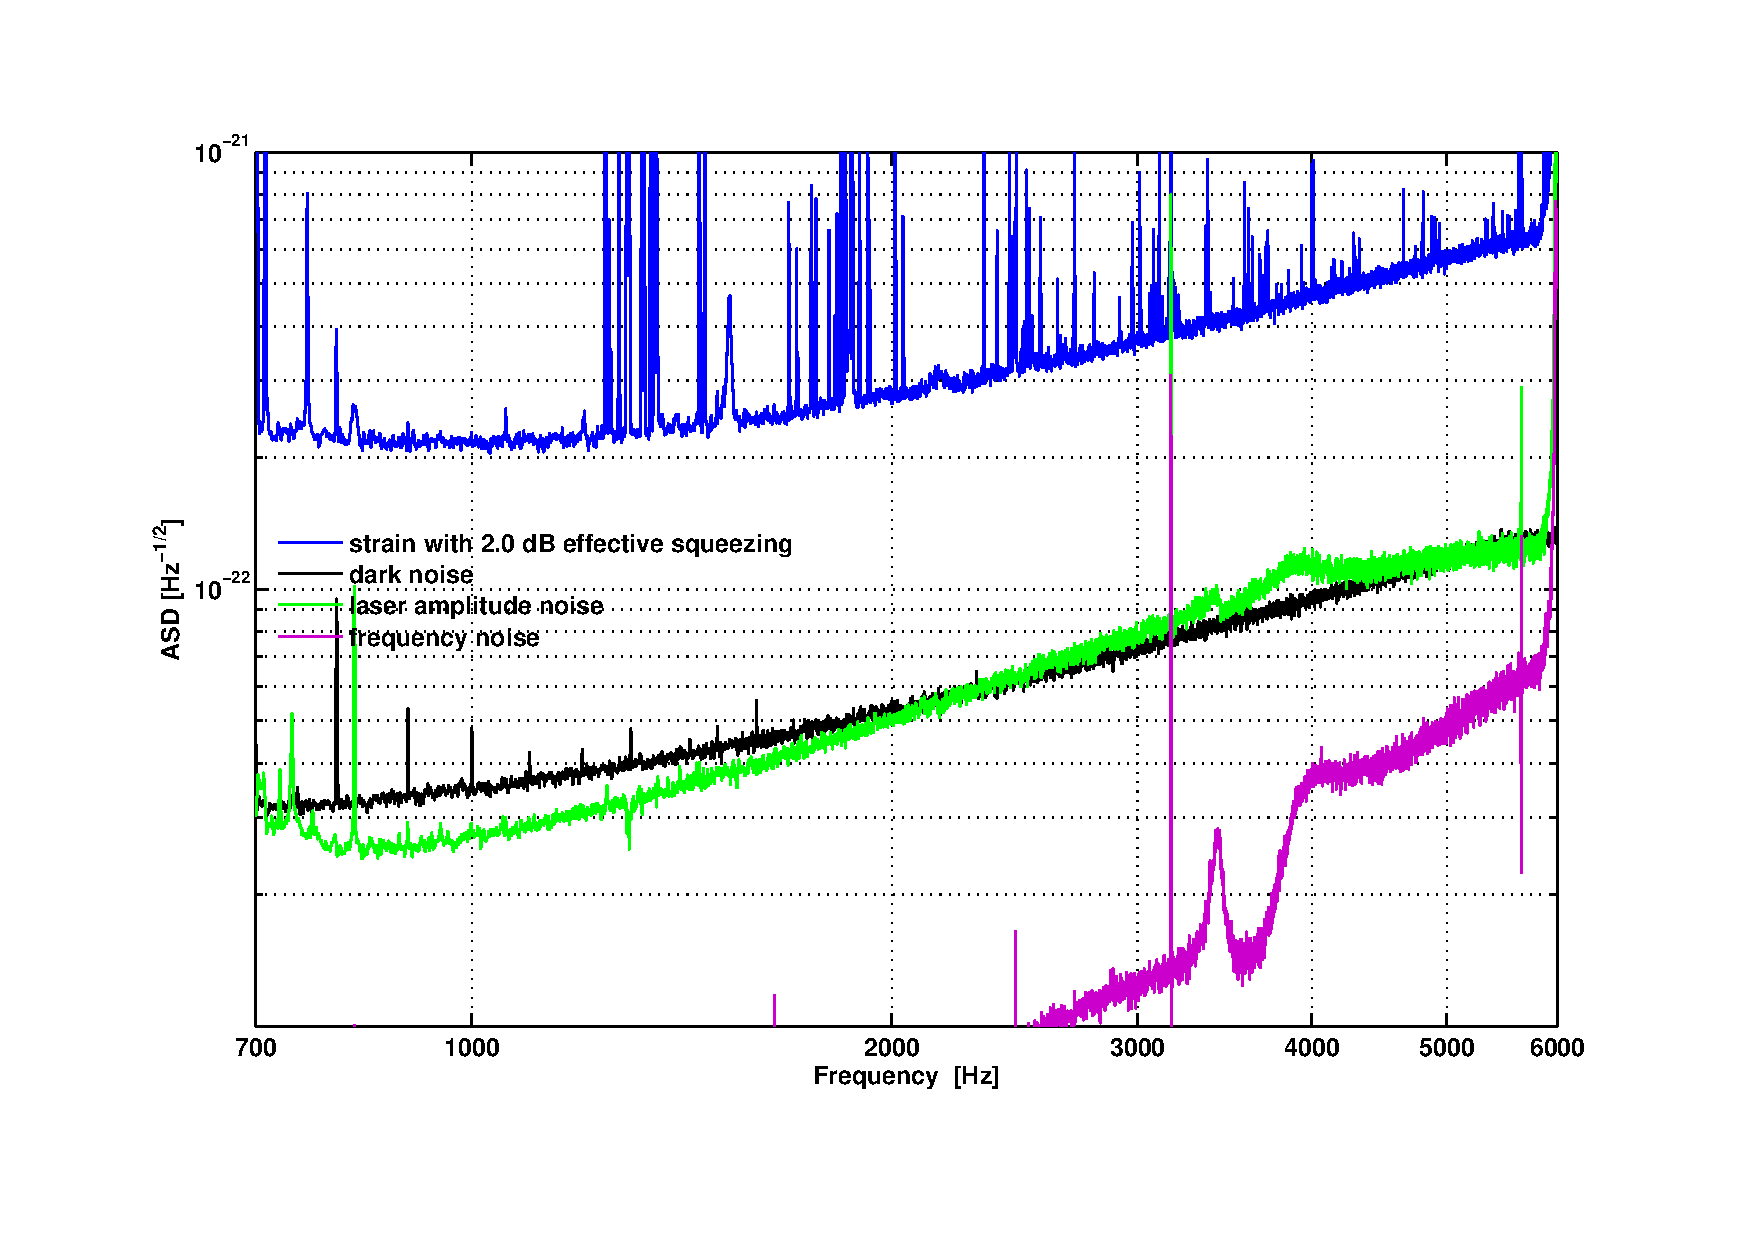
\includegraphics[width=1.0\textwidth]{/home/kadool/projects/GEOnoisebudget/HFnoise.pdf}
\caption{High frequency noises that result in a lower effective
  squeezing of strain than is actually achieved. In this example, shot
  noise is actually reduced by 2.4 dB due to squeezing, but the other
  noise sources, when added in quadrature with shot noise, reduce the
  effective squeezing to 2.0 dB. In this example, laser amplitude
  noise is abnormally high.}
\label{fig:HFnoises}
\end{centering}
\end{figure}


\section{Ideas for improvements}
\label{sec:future}

\begin{enumerate}
\item better OMC
\item 2 PDs for an on-board homodyne detector (?)
\item 2nd OMC
\end{enumerate}



\begin{table}
\centering
\caption{Optical losses of squeezed beam.}
\begin{tabular}{l l l l} %r@{}l r@{}l
\hline
component & power loss & 6-month goal \\
\hline
squeezer path Faraday & 3.3\% & 1.5\% \\
output port Faraday & 3.3\% $\times$ 2 & 1.5\% $\times$ 2 \\
BDO1 transmission & 1\% $\times$ 2 & 1\% $\times$ 2 \\
SR cavity (when locked) & 1\% & 1\% \\
OMC mode-matching loss & 6\% & 2\% \\
squeezer mode-matching loss & 2\% & 2\% \\
OMC AR coating loss & 1\% & 0.1\% \\
OMC internal losses & 14\% & 5\% \\
OMC trans PD detection loss & 9\% & 3\% \\
\hline
\end{tabular}
\label{tab:losses_goal}
\end{table}



\section{Acknowledgements}



\section{Appendix--OMC}
Table~\ref{tab:OMCparams} summarizes the current output mode cleaner
(OMC) design parameters. Note that the sideband transmission numbers
($T_{\mathrm{MI}}$ and $T_{\mathrm{SR}}$) should be doubled in
practice to account for the existence of both upper and lower
sidebands.

\begin{table}
\centering
\caption{OMC parameters. Many numbers come from p.12 of the GEO-HF logbook.}
\begin{tabular}{l l l l} %r@{}l r@{}l
\hline
quantity & symbol & value & units \\
\hline
Finesse & F & 160 & \\
round trip length & L & 0.658 & m \\
g-factor & g & 0.735 & \\
waist size & $\omega_0$ & 450 & \micro m \\
free spectral range & FSR & 455.6 & MHz \\
Michelson sideband frequency & $f_{\mathrm{MI}}$ & 14.90 & MHz \\
SRC sideband frequency & $f_{\mathrm{SR}}$ & 9.18 & MHz \\
Michelson sideband power transmission & $T_{\mathrm{MI}}$ & 1.01 & $\%$ \\
SRC sideband power transmission & $T_{\mathrm{SR}}$ & 2.71 & $\%$ \\
\hline
\end{tabular}
\label{tab:OMCparams}
\end{table}



\end{document}



